\chapter{Ledger Database}
\label{ledgerdb}

The Ledger DB is responsible for the following tasks:

\begin{enumerate}
\item \textbf{Maintaining the ledger state at the tip}: Maintaining the ledger
  state corresponding to the current tip in memory. When we try to extend our
  chain with a new block fitting onto our tip, the block must first be validated
  using the right ledger state, i.e., the ledger state corresponding to the tip.
  The current ledger state is needed for various other purposes.

\item \textbf{Maintaining the past $k$ ledger states}: As discussed in
  \cref{consensus:overview:k}, we might roll back up to $k$ blocks when
  switching to a more preferable fork. Consider the example below:
  %
  \begin{center}
  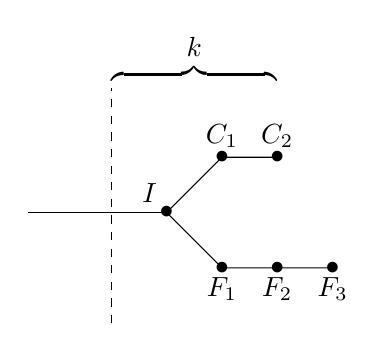
\begin{tikzpicture}
  \draw (0, 0) -- (50pt, 0) coordinate (I);
  \draw (I) -- ++(20pt,  20pt) coordinate (C1) -- ++(20pt, 0) coordinate (C2);
  \draw (I) -- ++(20pt, -20pt) coordinate (F1) -- ++(20pt, 0) coordinate (F2) -- ++(20pt, 0) coordinate (F3);
  \node at (I)  {$\bullet$};
  \node at (C1) {$\bullet$};
  \node at (C2) {$\bullet$};
  \node at (F1) {$\bullet$};
  \node at (F2) {$\bullet$};
  \node at (F3) {$\bullet$};
  \node at (I) [above left] {$I$};
  \node at (C1) [above] {$C_1$};
  \node at (C2) [above] {$C_2$};
  \node at (F1) [below] {$F_1$};
  \node at (F2) [below] {$F_2$};
  \node at (F3) [below] {$F_3$};
  \draw (60pt, 50pt) node {$\overbrace{\hspace{60pt}}$};
  \draw (60pt, 60pt) node[fill=white] {$k$};
  \draw [dashed] (30pt, -40pt) -- (30pt, 45pt);
  \end{tikzpicture}
  \end{center}
  %
  Our current chain's tip is $C_2$, but the fork containing blocks $F_1$, $F_2$,
  and $F_3$ is more preferable. We roll back our chain to the intersection point
  of the two chains, $I$, which must be not more than $k$ blocks back from our
  current tip. Next, we must validate block $F_1$ using the ledger state at
  block $I$, after which we can validate $F_2$ using the resulting ledger state,
  and so on.

  This means that we need access to all ledger states of the past $k$ blocks,
  i.e., the ledger states corresponding to the volatile part of the current
  chain.\footnote{Applying a block to a ledger state is not an invertible
  operation, so it is not possible to simply ``unapply'' $C_1$ and $C_2$ to
  obtain $I$.}

  Access to the last $k$ ledger states is not only needed for validating candidate
  chains, but also by the:
  \begin{itemize}
  \item \textbf{Local state query server}: To query any of the past $k$ ledger
    states (\cref{servers:lsq}).
  \item \textbf{Chain sync client}: To validate headers of a chain that
    intersects with any of the past $k$ blocks
    (\cref{chainsyncclient:validation}).
  \end{itemize}

\item \textbf{Storing on disk}: To obtain a ledger state for the current tip of
  the chain, one has to apply \emph{all blocks in the chain} one-by-one to the
  initial ledger state. When starting up the system with an on-disk chain
  containing millions of blocks, all of them would have to be read from disk and
  applied. This process can take tens of minutes, depending on the storage and
  CPU speed, and is thus too costly to perform on each startup.

  For this reason, a recent snapshot of the ledger state should be periodically
  written to disk. Upon the next startup, that snapshot can be read and used to
  restore the current ledger state, as well as the past $k$ ledger states.
\end{enumerate}

Note that whenever we say ``ledger state'', we mean the
\lstinline!ExtLedgerState blk! type described in \cref{storage:extledgerstate}.

The above duties are divided across the following modules:

\begin{itemize}
\item \lstinline!LedgerDB.InMemory!: this module defines a pure data structure,
  named \lstinline!LedgerDB!, to represent the last $k$ ledger states in memory.
  Operations to validate and append blocks, to switch to forks, to look up
  ledger states, \ldots{} are provided.
\item \lstinline!LedgerDB.OnDisk!: this module contains the functionality to
  write a snapshot of the \lstinline!LedgerDB! to disk and how to restore a
  \lstinline!LedgerDB! from a snapshot.
\item \lstinline!LedgerDB.DiskPolicy!: this module contains the policy that
  determines when a snapshot of the \lstinline!LedgerDB! is written to disk.
\item \lstinline!ChainDB.Impl.LgrDB!: this module is part of the Chain DB, and
  is responsible for maintaining the pure \lstinline!LedgerDB! in a
  \lstinline!StrictTVar!.
\end{itemize}

We will now discuss the modules listed above.

\section{In-memory representation}
\label{ledgerdb:in-memory}

The \lstinline!LedgerDB!, capable of represent the last $k$ ledger states, is an
instantiation of the \lstinline!AnchoredSeq! data type. This data type is
implemented using the \emph{finger tree} data structure~\cite{fingertrees} and
has the following time complexities:

\begin{itemize}
\item Appending a new ledger state to the end in constant time.
\item Rolling back to a previous ledger state in logarithmic time.
\item Looking up a past ledger state by its point in logarithmic time.
\end{itemize}

One can think of a \lstinline!AnchoredSeq! as a \lstinline!Seq! from
\lstinline!Data.Sequence! with a custom \emph{finger tree measure}, allowing for
efficient lookups by point, combined with an \emph{anchor}. When fully
\emph{saturated}, the sequence will contain $k$ ledger states. In case of a
complete rollback of all $k$ blocks and thus ledger states, the sequence will
become empty. A ledger state is still needed, i.e., one corresponding to the
most recent immutable block that cannot be rolled back. The ledger state at the
anchor plays this role.

When a new ledger state is appended to a fully saturated \lstinline!LedgerDB!,
the ledger state at the anchor is dropped and the oldest element in the sequence
becomes the new anchor, as it has become immutable. This maintains the invariant
that only the last $k$ ledger states are stored, \emph{excluding} the ledger
state at the anchor. This means that in practice, $k + 1$ ledger states will be
kept in memory. When fewer the \lstinline!LedgerDB! contains fewer than $k$
elements, new ones are appended without shifting the anchor until it is
saturated.

\todo{TODO} figure?

The \lstinline!LedgerDB! is parameterised over the ledger state $l$.
Conveniently, the \lstinline!LedgerDB! can implement the same abstract interface
(described in \cref{ledger:api}) that the ledger state itself implements. I.e.,
the \lstinline!GetTip!, \lstinline!IsLedger!, and \lstinline!ApplyBlock!
classes. This means that in most places, wherever a ledger state can be used, it
is also possible to wrap it in a \lstinline!LedgerDB!, causing it to
automatically maintain a history of the last $k$ ledger states.

\todo{TODO} discuss \lstinline!Ap! and \lstinline!applyBlock!? These are
actually orthogonal to \lstinline!LedgerDB! and should be separated.


\paragraph{Memory usage}

The ledger state is a big data structure that contains, amongst other things,
the entire UTxO. Recent measurements\footnote{Using the ledger state at the
block with slot number \num{16976076} and hash \lstinline!af0e6cb8ead39a86!.}
show that the heap size of an Allegra ledger state is around \num{361}~MB.
Fortunately, storing $k = \num{2160}$ ledger states in memory does \emph{not}
require $\num{2160} * \num{361}~\textrm{MB} = \num{779760}~\textrm{MB} =
\num{761}~\textrm{GB}$. The ledger state is defined using standard Haskell data
structures, e.g., \lstinline!Data.Map.Strict!, which are \emph{persistent} data
structures. This means that when we update a ledger state by applying a block to
it, we only need extra memory for the new and the modified data. The majority of
the data will stay the same and will be \emph{shared} with the previous ledger
state.

The memory required for storing the last $k$ ledger state is thus proportional
to: the size of the oldest in-memory ledger state \emph{and} the changes caused
by the last $k$ blocks, e.g., the number of transactions in those blocks.
Compared to the \num{361}~MB required for a single ledger state, keeping the
last $k$ ledger states in memory requires only \num{375}~MB in total. This is
only \num{14}~MB or 3.8\% more memory. Which is a very small cost.

\paragraph{Past design}

In the past, before measuring this cost, we did not keep all $k$ past ledger
states because of an ungrounded fear for the extra memory usage. The
\lstinline!LedgerDB! data structure had a \lstinline!snapEvery! parameter,
ranging from 1 to $k$, indicating that a snapshot, i.e., a ledger state, should
be kept every \lstinline!snapEvery! ledger states or blocks. In practice, a
value of 100 was used for this parameter, resulting in 21--22 ledger states in
memory.

The representation was much more complex, to account for these missing ledger
states. More importantly, accessing a past ledger state or rewinding the
\lstinline!LedgerDB! to a past ledger state had a very different cost model. As
the requested ledger state might not be in memory, it would have to be
\emph{reconstructed} by reapplying blocks to an older ledger state.

Consider the example below using \lstinline!snapEvery! = 3. $L_i$ indicate
ledger states and $\emptyset_i$ indicate skipped ledger states. $L_0$ corresponds to the
most recent ledger state, at the tip of the chain.
%
\begin{center}
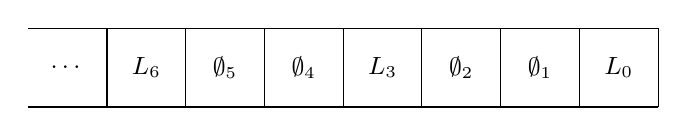
\begin{tikzpicture}
\draw (0, 0) -- (8, 0);
\draw (0, 1) -- (8, 1);

\draw (1, 0) -- (1, 1);
\draw (2, 0) -- (2, 1);
\draw (3, 0) -- (3, 1);
\draw (4, 0) -- (4, 1);
\draw (5, 0) -- (5, 1);
\draw (6, 0) -- (6, 1);
\draw (7, 0) -- (7, 1);
\draw (8, 0) -- (8, 1);

\draw (0.5, 0.5) node {\small \ldots};
\draw (1.5, 0.5) node {\small $L_6$};
\draw (2.5, 0.5) node {\small $\emptyset_5$};
\draw (3.5, 0.5) node {\small $\emptyset_4$};
\draw (4.5, 0.5) node {\small $L_3$};
\draw (5.5, 0.5) node {\small $\emptyset_2$};
\draw (6.5, 0.5) node {\small $\emptyset_1$};
\draw (7.5, 0.5) node {\small $L_0$};

\end{tikzpicture}
\end{center}
%
When we need access to the ledger state at position $3$, we are in luck and can
use the available $L_3$. However, when we need access to the skipped ledger
state at position $1$, we have to do the following: we look for the most recent
ledger state before $\emptyset_1$, i.e., $L_3$. Next, we need to reapply blocks $B_2$
and $B_1$ to it, which means we have to read those from disk, deserialise them,
and apply them again.

This means that accessing a past ledger state is not a pure operation and might
require disk access and extra computation. Consequently, switching to a fork
might require reading and revalidating blocks that remain part of the chain, in
addition to the new blocks.

As mentioned at the start of this chapter, the chain sync client also needs
access to past ledger view (\cref{consensus:class:ledgerview}), which it can
obtain from past ledger states. A malicious peer might try to exploit it and
create a chain that intersects with our chain right \emph{before} an in-memory
ledger state snapshot. In the worst case, we have to read and reapply
\lstinline!snapEvery! - 1 = 99 blocks. This is not acceptable as the costs are
asymmetric and in the advantage of the attacker, i.e., creating and serving such
a header is much cheaper than reconstructing the required snapshot. At the time,
we solved this by requiring ledger states to store snapshots of past ledger
views. The right past ledger view could then be obtained from the current ledger
state, which was always available in memory. However, storing snapshots of
ledger views within a single ledger state is more complex, as we are in fact
storing snapshots \emph{within} snapshots. The switch to keep all $k$ past
ledger states significantly simplified the code and sped up the look-ups.

\paragraph{Future design}

It is important to note that in the future, this design will have to change
again. The UTxO and, consequently, the ledger state are expected to grow in size
organically. This growth will be accelerated by new features added to the
ledger, e.g., smart contracts. At some point, the ledger state will be so large
that keeping it in its entirety in memory will no longer be feasible. Moreover,
the cost of generating enough transactions to grow the current UTxO beyond the
expected memory limit might be within reach for some attackers. Such an attack
might cause a part of the network to be shut down because the nodes in question
are no longer able to load the ledger state in memory without running against
the memory limit.

For these reasons, we plan to revise our design in the future, and start storing
parts of the ledger state on disk again.

\section{On-disk}
\label{ledgerdb:on-disk}

The \lstinline!LedgerDB.OnDisk! module provides functions to write a ledger
state to disk and read a ledger state from disk. The \lstinline!EncodeDisk! and
\lstinline!DecodeDisk! classes from \cref{serialisation:storage} are used to
(de)serialise the ledger state to or from CBOR. Because of its large size, we
read and deserialise the snapshot incrementally.

\todo{TODO} which ledger state to take a snapshot from is determined by the
Chain DB. I.e., the background thread that copies blocks from the Volatile DB to
the Immutable DB will call the \lstinline!onDiskShouldTakeSnapshot! function,
and if it returns \lstinline!True!, a snapshot will be taken. \todo{TODO}
double-check whether we're actually taking a snapshot of the right ledger state.

\subsection{Disk policy}
\label{ledgerdb:on-disk:disk-policy}

The disk policy determines how many snapshots should be stored on disk and when
a new snapshot of the ledger state should be written to disk.

\todo{TODO} worth discussing? We would just be duplicating the existing
documentation.

\subsection{Initialisation}
\label{ledgerdb:on-disk:initialisation}

During initialisation, the goal is to construct an initial \lstinline!LedgerDB!
that is empty except for the ledger state at the anchor, which has to correspond
to the immutable tip, i.e., the block at the tip of the Immutable DB
(\cref{immutable}).

Ideally, we can construct the initial \lstinline!LedgerDB! from a snapshot of
the ledger state that we wrote to disk. Remember that updating a ledger state
with a block is not invertible: we can apply a block to a ledger state, but we
cannot ``unapply'' a block to a ledger state. This means the snapshot has to be
at least as old as the anchor. A snapshot matching the anchor can be used as is.
A snapshot older than the anchor can be used after reapplying the necessary
blocks. A snapshot newer than the anchor can \emph{not} be used, as we cannot
unapply blocks to get the ledger state corresponding to the anchor. This is the
reason why we only take snapshots of an immutable ledger state, i.e., of the
anchor of the \lstinline!LedgerDB! (or older).

Constructing the initial \lstinline!LedgerDB! proceeds as follows:
\begin{enumerate}
\item If any on-disk snapshots are available, we try them from new to old. The
  newer the snapshot, the fewer blocks will need to be reapplied.
\item We deserialise the snapshot. If this fails, we try the next one.
\item If the snapshot is of the ledger state corresponding to the immutable tip,
  we can use the snapshot for the anchor of the \lstinline!LedgerDB! and are
  done.
\item If the snapshot is newer than the immutable tip, we cannot use it and try
  the next one. This situation can arise not because we took a snapshot of a
  ledger state newer than the immutable tip, but because the Immutable DB was
  truncated.
\item If the snapshot is older than the immutable tip, we will have to reapply
  the blocks after the snapshot to obtain the ledger state at the immutable tip.
  If there is no (more) snapshot to try, we will have to reapply \emph{all
  blocks} starting from the beginning of the chain to obtain the ledger state at
  the immutable tip, i.e., the entire immutable chain. The blocks to reapply are
  streamed from the Immutable DB, using an iterator
  (\cref{immutable:api:iterators}).

  Note that we can \emph{reapply} these blocks, which is quicker than applying
  them (see \cref{ledgerdb:lgrdb}), as the existence of a snapshot newer than
  these blocks proves\footnote{Unless the on-disk database has been tampered
  with, but this is not an attack we intend to protect against, as this would
  mean the machine has already been compromised.} that they have been
  successfully applied in the past.
\end{enumerate}
%
Reading and applying blocks is costly. Typically, very few blocks need to be
reapplied in practice. However, there is one exception: when the serialisation
format of the ledger state changes, all snapshots (written using the old
serialisation format) will fail to deserialise, and all blocks starting from
genesis will have to be reapplied. To mitigate this, the ledger state decoder is
typically written in a backwards-compatible way, i.e., it accepts both the old
and new serialisation format.

\section{Maintained by the Chain DB}
\label{ledgerdb:lgrdb}

\todo{TODO} move to Chain DB chapter?

The \lstinline!LedgerDB! is a pure data structure. The Chain DB (see
\cref{chaindb}) maintains the current \lstinline!LedgerDB! in a
\lstinline!StrictTVar!. The most recent element in the \lstinline!LedgerDB! is
the current ledger state. Because it is stored in a \lstinline!StrictTVar!, the
current ledger state can be read and updated in the same \lstinline!STM!
transaction as the current chain, which is also stored in a
\lstinline!StrictTVar!.

The \lstinline!ChainDB.Impl.LgrDB!\footnote{In the past, we had similar modules
for the \lstinline!VolatileDB! and \lstinline!ImmutableDB!, i.e.,
\lstinline!VolDB! and \lstinline!ImmDB!. The former were agnostic of the
\lstinline!blk! type and the latter instantiated the former with the
\lstinline!blk! type. However, in hindsight, unifying the two proved to be
simpler and was thus done. The reason why a separate \lstinline!LgrDB! still
exists is mainly because it needs to wrap the pure \lstinline!LedgerDB! in a
\lstinline!StrictTVar!.} is responsible for maintaining the current ledger
state. Besides this responsibility, it also integrates the Ledger DB with other
parts of the Chain DB.

Moreover, it remembers which blocks have been successfully applied in the past.
When such a block needs to be validated again, e.g., because we switch again to
the same fork containing the block, we can \emph{reapply} the block instead of
\emph{applying} it (see \cref{ledger:api:ApplyBlock}). Because the block has
been successfully applied in the past, we know the block is valid, which means
we can skip some of the more expensive checks, e.g., checking the hashes,
speeding up the process of validating the block. Note that a block can only be
applied to a single ledger state, i.e., the ledger state corresponding to the
predecessor of the block. Consequently, it suffices to remember whether a block
was valid or not, there is no need to remember with respect to which ledger
state it was valid.

To remember which blocks have been successfully applied in the past, we store
the points of the respective blocks in a set. Before validating a block, we look
up its point in the set, when present, we can reapply the block instead of
applying it. To stop this set from growing without bound, we garbage collect it
the same way the Volatile DB is garbage collected, see \cref{chaindb:gc}. When a
block has a slot older than the slot number of the most recent immutable block,
either the block is already immutable or it is part of a fork that we will never
consider again, as it forks off before the immutable block.\todo{slot number vs
  block number} The block in question will never have to be validated again, and
so it is not necessary to remember whether we have already applied it or not.
